\chapter{Switching}

\section{Circuit Switching}
Circuit switching is a method of communication that involves three main phases:

\subsubsection{Establishing a Circuit}
\begin{itemize}
   \item A logical connection is created between the two endpoints.
   \item A dedicated path is established for data transmission.
   \item Resources at intermediate switches are reserved for the duration of the communication.
\end{itemize}

\subsubsection{Transferring the Data}
\begin{itemize}
   \item Once the connection is established, the entire data stream travels over the dedicated path from the sender to the receiver.
\end{itemize}

\subsubsection{Disconnecting the Circuit}
\begin{itemize}
   \item After the data transfer is complete, the established connection is disconnected.
\end{itemize}

\vspace{2ex}
\begin{figure}[th]
   \centering
   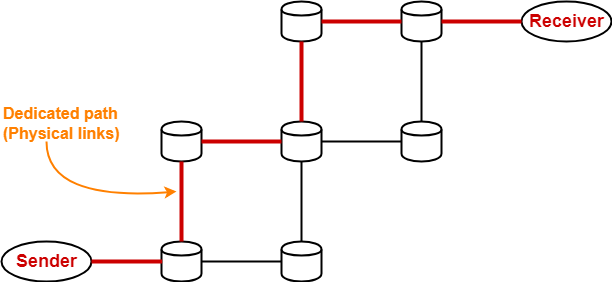
\includegraphics[width=0.5\textwidth]{figures/Circuit Switching.png}
   \caption{Circuit Switching}
\end{figure}

\section{Packet Switching}
Packet switching enhances efficiency and flexibility in data transmission by utilizing the network's resources more effectively.

\subsubsection{Process of Packet Switching}
\begin{itemize}
   \item The complete message is divided into smaller packets in a process called packetization.
   \item These smaller packets are transmitted individually over the network, allowing them to take different paths to the destination.
   \item This method enables pipelining, which reduces the overall transmission time for the entire message.
\end{itemize}

\vspace{2ex}
\begin{figure}[th]
   \centering
   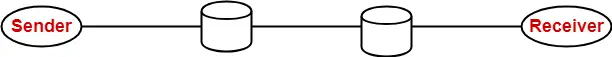
\includegraphics[width=0.5\textwidth]{figures/Packet Switching.png}
   \caption{Packet Switching}
\end{figure}


\begin{center}
   \large
   \textbf{Formula Sheet}
\end{center}

% \subsection*{Circuit Switching}

\vspace{5ex}
$\begin{aligned}
& \text{5 MB} = \text{5} \times \text{1024} \times \text{1024} \times \text{8 bits \, (exact)} = \text{5} \times \text{10}^{\text{6}} \times \text{8 bits \, (approx)} \\[3ex]
& \text{Transmission delay} = \frac{\text{File Size (bits)}}
{\text{Data Rate (bps)}} \\[3ex]
& \text{Queuing delay} =
\frac{\text{Final queue size}-\text{Initial queue size}}
{\text{Packets arriving per second - Packets processed per second}}\\[3ex]
& \text{Propagation delay} =
\frac{\text{Distance}}{\text{Propagation Speed}} \\[3ex]
& T_\text{total}
= T_\text{Transmission} + \left[(T_\text{Queue}
+ T_\text{Processing} + T_\text{Propagation}) \times \text{Number of hops} \right]\\[3ex]
\end{aligned}$